\documentclass[10pt,a4paper]{report}
\usepackage[utf8]{inputenc}
\usepackage{url}
\usepackage[english]{babel}
\usepackage{amsmath}
\usepackage{amsfonts}
\usepackage{amssymb}
\usepackage{listings}
 \usepackage{float}
\usepackage{graphicx}
\usepackage[left=2cm,right=2cm,top=2cm,bottom=2cm]{geometry}
\author{Andres Chaves}
\title{Report 1: Data Analysis}

\begin{document}
 \title{Report 1: Data Description and Analysis}
 \author{Andres Chaves (706801) \\
  \multicolumn{1}{p{.7\textwidth}}{\centering{achaves@student.unimelb.edu.au\\}\centering\emph{Melbourne School of Information\\The University of Melbourne}}}
 \maketitle

\begin{abstract}
    The purpose of this document is to describe and analyse the available data from which the experiments will be executed.
   \\\\
   Throughout this document we will understand what is the data, how the data is generated, received, stored and how much is available. We will see also some examples of relations between the data.
\end{abstract}

 \chapter*{Introduction}
The objective of my Research Project is to explore how Machine Learning technologies can be used for aid the Network Management process, specifically the Fault Management process. 
\\\\
One of the key Information Technology components in Fault Management is the Fault  Management System (FMS). A FMS is a system that receives all the alarms from the different Network Elements (NEs), performs several data transformations, and at the end stores enriched alarms and allows their visualisation:

\begin{figure}[H]
 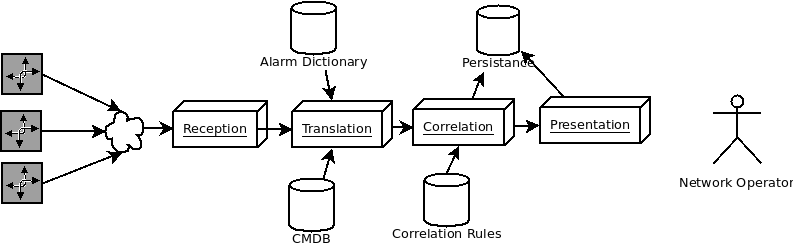
\includegraphics[scale=0.4]{../research_proposal/NMS_GeneralDiagram.png}
  \centering
  \caption{\textit{A schematic of a generic Fault Management System}}
  \label{fig:nms_generaldiagram}
\end{figure}	

The processing stages might include the following steps:

\begin{itemize}
\item Translation: Consist on receive the alarm in a given standard, de-codify it, translate it and enrich it into useful data. This is a required step.

\item Correlation: Consist on establish rules for alarm suppression and correlation to present only key information to the network operator.
\end{itemize}

The proposed hypothesis of my Research is that given an alarm of interest an unsupervised learning algorithm can be run in order to find correlation between the alarm of interest and other alarms and therefore suppress the related alarms.
\\\\
In order to conduct the experiments and analysis required for evaluating the hypothesis, it is required to have a data set from a FMS. For the scope of this project I will use the data from one FMS built in a company I worked on in the past.
\\\\
We will see an introduction to the Simple Network Management Protocol(SNMP) and then some details of the specific FMS along with some insight on the network that is managed by this system. Finally, we will analyse the data by proposing five possible correlation rules.

\chapter{Simple Network Management Protocol}
SNMP is a Layer 7 Network Protocol, specified in 1990 by the IETF, created to standardise a way to manage Network Elements. In this management protocol there are five message types and four of these are based on Request-Response interaction between a Network Management System (NMS) and a NE: GetRequest-PDU, GetNextRequest-PDU, GetResponse-PDU, SetRequest-PDU. With these four message types a NMS can read either a value or a set of values an also can write a value to override parts of the configuration of the NE. The full details of the protocol can be reviewed in RFC 1157\cite{snmp}.
\\\\
The fifth message type, named Trap-PDU, allows a Network Element to inform the NMS about significant events or alarms in an unsolicited and asynchronous way\cite{ciscoTraps}. This is the key mechanism of a typical Fault Management System.
\\\\
The alarms can be either generic ones, specified by the protocol, or specific enterprise ones. Each alarm type has a specific Object Identifier (OID) to allow the system the identification of the alarm. Alarms can also have zero or more variables bindings according to the alarm type.
\\\\
The set of alarm types that a given equipment can send is described in the Management Information Base (MIB) which is a collection of ASN.1 files that specify all the possible alarm types, measurements and configuration values that can be managed in the network element.
\\\\
The following figure summarises the SNMP Trap mechanism:
\\\\
\begin{figure}[H]
 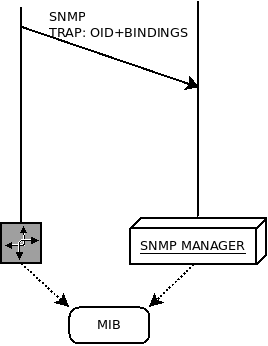
\includegraphics[scale=0.4]{SNMP_Trap.png}
  \centering
  \caption{\textit{A representation of the SNMP Trap message}}
  \label{fig:snmp_trap}
\end{figure}	

\newpage
As an example of MIB specification we can see a definition of the LinkDown alarm specified by Cisco equipment vendor in CISCOGENERAL-MIB\cite{ciscoGeneralTraps}:

\begin{figure}[H]
 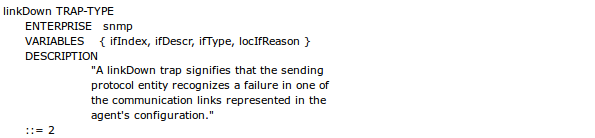
\includegraphics[scale=0.4]{ciscoTrapLinkDown.png}
  \centering
  \caption{\textit{Cisco Trap Specification}}
  \label{fig:snmp_mib_example}
\end{figure}	

This LinkDown alarm specified in the example has the OID .1.3.6.1.2.1.11.0.3 and four variable bindings: ifIndex, ifDesccr, ifType and locIfReason.

\chapter{Fault Management System}

Based on the overall components of a generic FMS in Figure \ref{fig:nms_generaldiagram} and using the SNMP protocol, we built in the company a specific FMS using several Open Source software. A schematic of the FMS, with all the open source components, can be seen in this figure:

\begin{figure}[H]
 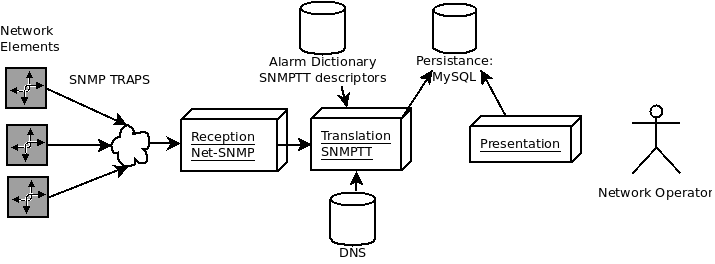
\includegraphics[scale=0.4]{ACC_FMS.png}
  \centering
  \caption{\textit{Our built Fault Network Management System}}
  \label{fig:acc_fms}
\end{figure}	


The FMS receives alarms using the SNMP protocol. The Open Source components used are described as follows:

\begin{itemize}
  \item Net-SNMP: Net-SNMP is an open source Linux and Unix package that implements the SNMP protocol. The role of this component will be the reception of alarms by using the snmptrapd daemon\cite{netsnmp}.
  \item SNMPTT: SNMPTT or SNMP-Trap Translator is an open source component that takes the SNMP trap (alarm) received by Net-SNMP and by using an alarm dictionary (to interpret the alarm name and its attributes) and a DNS (to gather the NE name) translates it into a more useful event. SNMPTT can also enrich the alarm from a database by executing a shell script.\cite{snmptt}
  \item MYSQL: MySQL is an open source relational database. For this FMS, it was used for the storage of the Alarms\cite{mysql}.
\end{itemize}

\chapter{Network Description}
In order to understand the scenarios and alarms that arrive to the FMS described in the last chapter, it is important to have an overview of the network managed by the FMS. The purpose of this chapter is to outline this network.
\\\\
The network is designed hierarchically based on the Cisco hierarchical (three-layer) internetworking model\cite{ciscoNetworkDesign}:

\begin{figure}[H]
 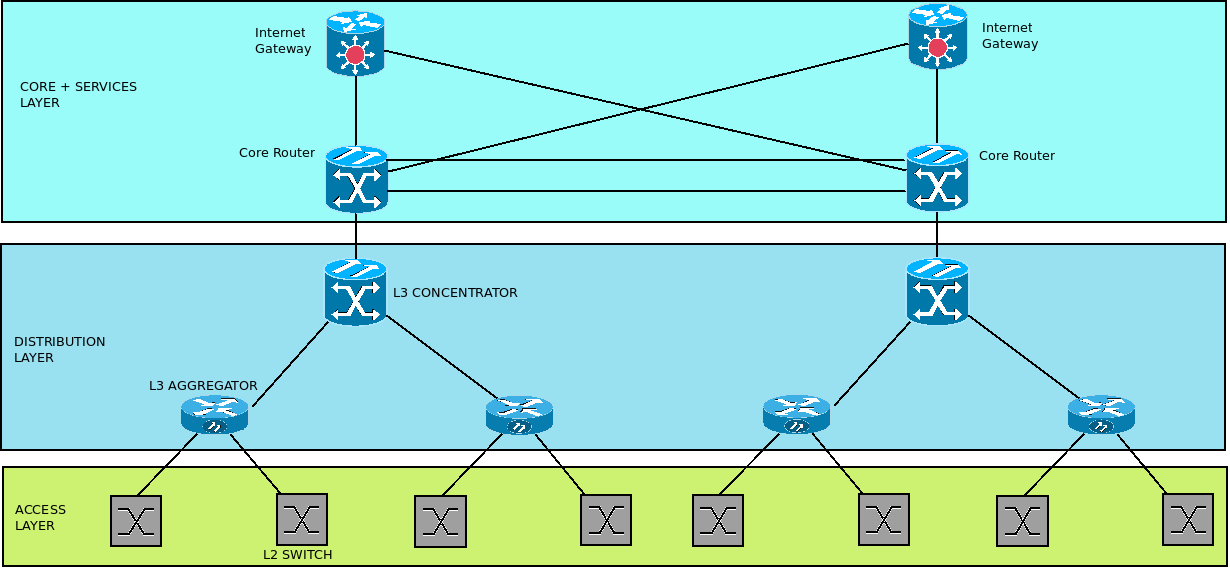
\includegraphics[scale=0.4]{Network_Architecture.png}
  \centering
  \caption{\textit{Network Design}}
  \label{fig:network_design}
\end{figure}	

It is important to mention that there are two different equipment vendors distributed geographically.

\subsection{Access Layer}
Correspond to the Layer 2 switching layer. The last miles and client services are connected to this layer. The most significant equipment of this layer is the Switch.
\\\\
This is the bigger layer in terms of number of network elements, as in every town/city there should be at least one equipment. The switch is installed in an Access Node which can be thought as a small location/rack. The node is supported by a battery bank connected to a Rectifier element that converts AC to DC.
\\\\
The switch has both 10G and 1G ports. The 10G optical ports are use to connect the location to a higher hierarchical equipment. The 1G ports are used to provide all the services in the town. Normally last mile equipments, such as Wifi or PointToMultiPoint (PMP) radios, are connected to these ports.
\\\\
The following figure illustrates the key components on an access node:
\begin{figure}[H]
 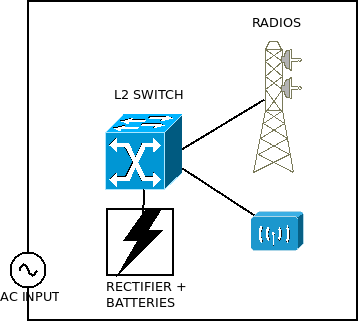
\includegraphics[scale=0.4]{access_node.png}
  \centering
  \caption{\textit{Schematic of an access node}}
  \label{fig:network_design}
\end{figure}	


\subsection{Distribution Layer}
Correspond to the Layer 3 Distribution layer. In this layer we have Routers that aggregate the traffic of several nodes and convert the Layer 2 domain into Layer 3. There are two types of node in this layer: the Aggregator node which correspond to a medium sized town that connects between 10 and 50 access nodes, and the Concentrator node which normally contains a bigger router and is installed in the main city of the state and process all the traffic in the region.

\subsection{Core Layer+Internet Gateway}
This layer is composed by big MPLS routers in charge of packet switching between all the concentrators and the different Internet Gateways or Data center services (broadband, tv, telephony, etc). These equipments are normally installed in datacenters.

\subsection{Host Naming Convention}
It is important to describe the host naming convention used for the network elements because it provides useful information. A host name is a 19 character string which follows the convention NEROLE\_BRAND\_MODEL\_STATE\_TOWN\_CONSECUTIVE (i.e: AC\_ER\_SP10\_ST\_VCH\_1):

\begin{itemize}
   \item Network Element Role: Two letters that correspond to the type of node where the network element is located. The type of node can be AC (Access), AG (Aggregator), CN (Concentrator), CR (CORE), IG (Internet Gateway) and RC (Rectifier).
   \item Brand: Two letters that correspond to the vendor of the equipment. Some examples are: ER, AL, DT.
   \item Model: Four letters that codify the NE's model. Some examples are: SP10, SA30, DP29.
   \item State: Two letters that represent the state where the network element is physically located.
   \item Town: Three letters encoding the town where the network element is physically located.
\end{itemize}

 
\chapter{Data Specification}

The FMS described in Chapter 2 stores the alarms in a table on a Relational Database System. Each month of alarms is stored in a separated table. For the purpose of this analysis we used the table for the month of October, 2014.

\section{Data Attributes}

The relevant attributes of the alarms stored are:

\begin{itemize}
  \item Id: Unique numeric identifier of each alarm.
  \item Eventname: Correspond to the translated name of the alarm's OID as informed by the SNMPTT dictionary.
  \item Traptime: Timestamp of arrival of the trap.
  \item Hostname: Ip or host name of the entity that sends the alarm. A DNS is queried in order to translate the IP Address, if the translation is successful the name is stored otherwise the ip is inserted. 
  \item Formatline: Semi-structured formatted line of the alarm. Normally it includes all the alarm's trap bindings.
\end{itemize}

\begin{figure}[H]
 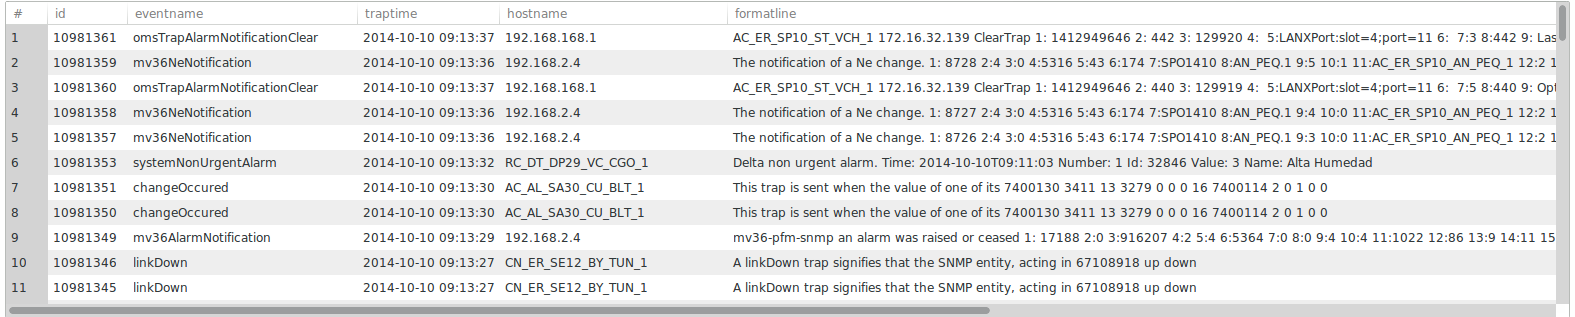
\includegraphics[scale=0.4]{alarms_db_sample.png}
  \centering
  \caption{\textit{An example of the stored data}}
  \label{fig:acc_dataexample}
\end{figure}	

\section{Data Overview} 
For the particular month of October 2014 we have the following statistics:

\begin{center}
 \begin{tabular}{||c | c ||} 
 \hline\hline
 Total Alarms  & 2350714 \\ 
 \hline
 Different Alarm Types & 351 \\ 
 \hline
 Different Host Names & 3272 \\
  \hline
 Average of Alarms Received per Minute & 53 \\
 \hline
 Peak of Alarms Received in a Minute & 714 \\
 \hline\hline
\end{tabular}
\end{center}

\section{Data Analysis} 
In order to have a better insight of the data and to understand better what should be the work required by the learning algorithm, we will describe 5 different scenarios of correlation between two alarms.
\\\\
For each correlation scenario we calculated the following: given in a time window of 1 minute, what is the probability of occurrence of the target alarm $a_t$, the probability of the second alarm $a_i$ and the conditional probability of the alarm $a_i$ given the occurrence of the alarm $a_t$.

\subsection{Scenario 1: AC Outage + Link Down, Vendor 1}
As stated in Chapter 3, the access node is composed by a Layer 2 equipment, a rectifier, a battery set, and possibly with several radios for the last miles. The radios are connected to the Ethernet ports of the switch.
\\\\
The power source of the radios can be DC or AC, if it is DC and there is an AC Outage the radio will be backed up by the battery bank. Conversely, if the power source is AC and there is an AC Outage the radio will turn off and the switch equipment will register a LinkDown trap.
\\\\
Therefore, the proposed scenario is the following: For vendor 1, given an AC Outage Alarm in a given town, it is expected to receive a LinkDown trap from the given town within the specified time window.

\subsection{Scenario 2: AC Recovery + Link Up, Vendor 1} 
As stated in the last scenario, if the radio was connected using an AC power source, it is expected that when the AC power is restored, the radio will power on and the switch will send a LinkUp trap.
\\\\
Specifically, the proposed scenario is the following: For vendor 1, given an AC Recovery Alarm in a given town, it is expected to receive a LinkUp trap from the given town within the specified time window.

\subsection{Scenario 3: AC Outage + Link Down, Vendor 2} 
This is the same Scenario 1, applied to the second vendor

\subsection{Scenario 4: AC Recovery + Link Up, Fabricator 2} 

This is the same Scenario 2, applied to the second vendor

\subsection{Scenario 5: Fuse Breaker Alarm + Link Down, Vendor 1} 
The rectifier in the node is a smart equipment that can detect when a breaker opens in the energy distribution chain inside the node.
\\\\
The last scenario analysed is the following: Given a breaker open alarm from the rectifier, it is expected to receive a LinkDown within the specified time window.

\subsection{Summary}

The following table summarises the frequencies:

\begin{center}
 \begin{tabular}{||c | c | c | c ||} 
 \hline\hline
 Scenario  & $P_t(a_t)$ & $P_t(a_i)$ & $P_t(a_i|a_t)$ \\ 
 \hline
 AC Outage + Link Down Vendor 1 & 0.2214 & 0.3886 & 0.11 \\  
 \hline
 AC Recovery + Link Up Vendor 1 & 0.1990 & 0.1228 & 0.117 \\  
 \hline
 AC Outage + Link Down Vendor 2 & 0.0421 & 0.6704 & 0.407 \\  
 \hline
 AC Outage + Link Up Vendor 2 & 0.0443 & 0.6645 & 0.366 \\  
 \hline
 Fuse Alarm + Link Down Vendor 2 & 0.0272 & 0.6704 & 0.027 \\  

 \hline\hline
\end{tabular}
\end{center}


 \begin{thebibliography}{9}
\bibitem{snmp}IETF RFC 1157, \url{http://www.ietf.org/rfc/rfc1157.txt?number=1157}.
\bibitem{ciscoTraps}Cisco Traps Documentation, \url{http://www.cisco.com/c/en/us/support/docs/ip/simple-network-management-protocol-snmp/7244-snmp-trap.html}.
\bibitem{ciscoGeneralTraps}Cisco General Trap MIB, \url{http://tools.cisco.com/Support/SNMP/do/BrowseMIB.do?local=en&step=2&submitClicked=true&mibName=CISCO-GENERAL-TRAPS}
\bibitem{netsnmp}Net-SNMP website, \url{http://www.net-snmp.org/}.
\bibitem{snmptt}SNMPTT website, \url{http://snmptt.sourceforge.net/docs/snmptt.shtml}.
\bibitem{mysql}MySQL website, \url{http://dev.mysql.com/doc/refman/4.1/en/what-is-mysql.html}.
\bibitem{ciscoNetworkDesign}Cisco Networking Academy Connecting Networks Companion Guide: Hierarchical Network Design, \url{http://www.ciscopress.com/articles/article.asp?p=2202410}

 
\end{thebibliography}
    
\end{document}
